\chapter{System Design}

\section{Overview}
In this section, we will illustrate the entire system in detail. We will go through all the various technologies that were finalized from the technical review, where they are located in the project structure and what role they have in creating a fluid and realistic experience for the user. In Figure~\ref{image:SystemArch} we can see the high-level design of the project. Each component has a major roll to play in creating this fluid experience and we will discuss how they where implemented now in detail.

\begin{figure}[h!]
	\caption{System Architecture.}
	\label{image:SystemArch}
	\centering
	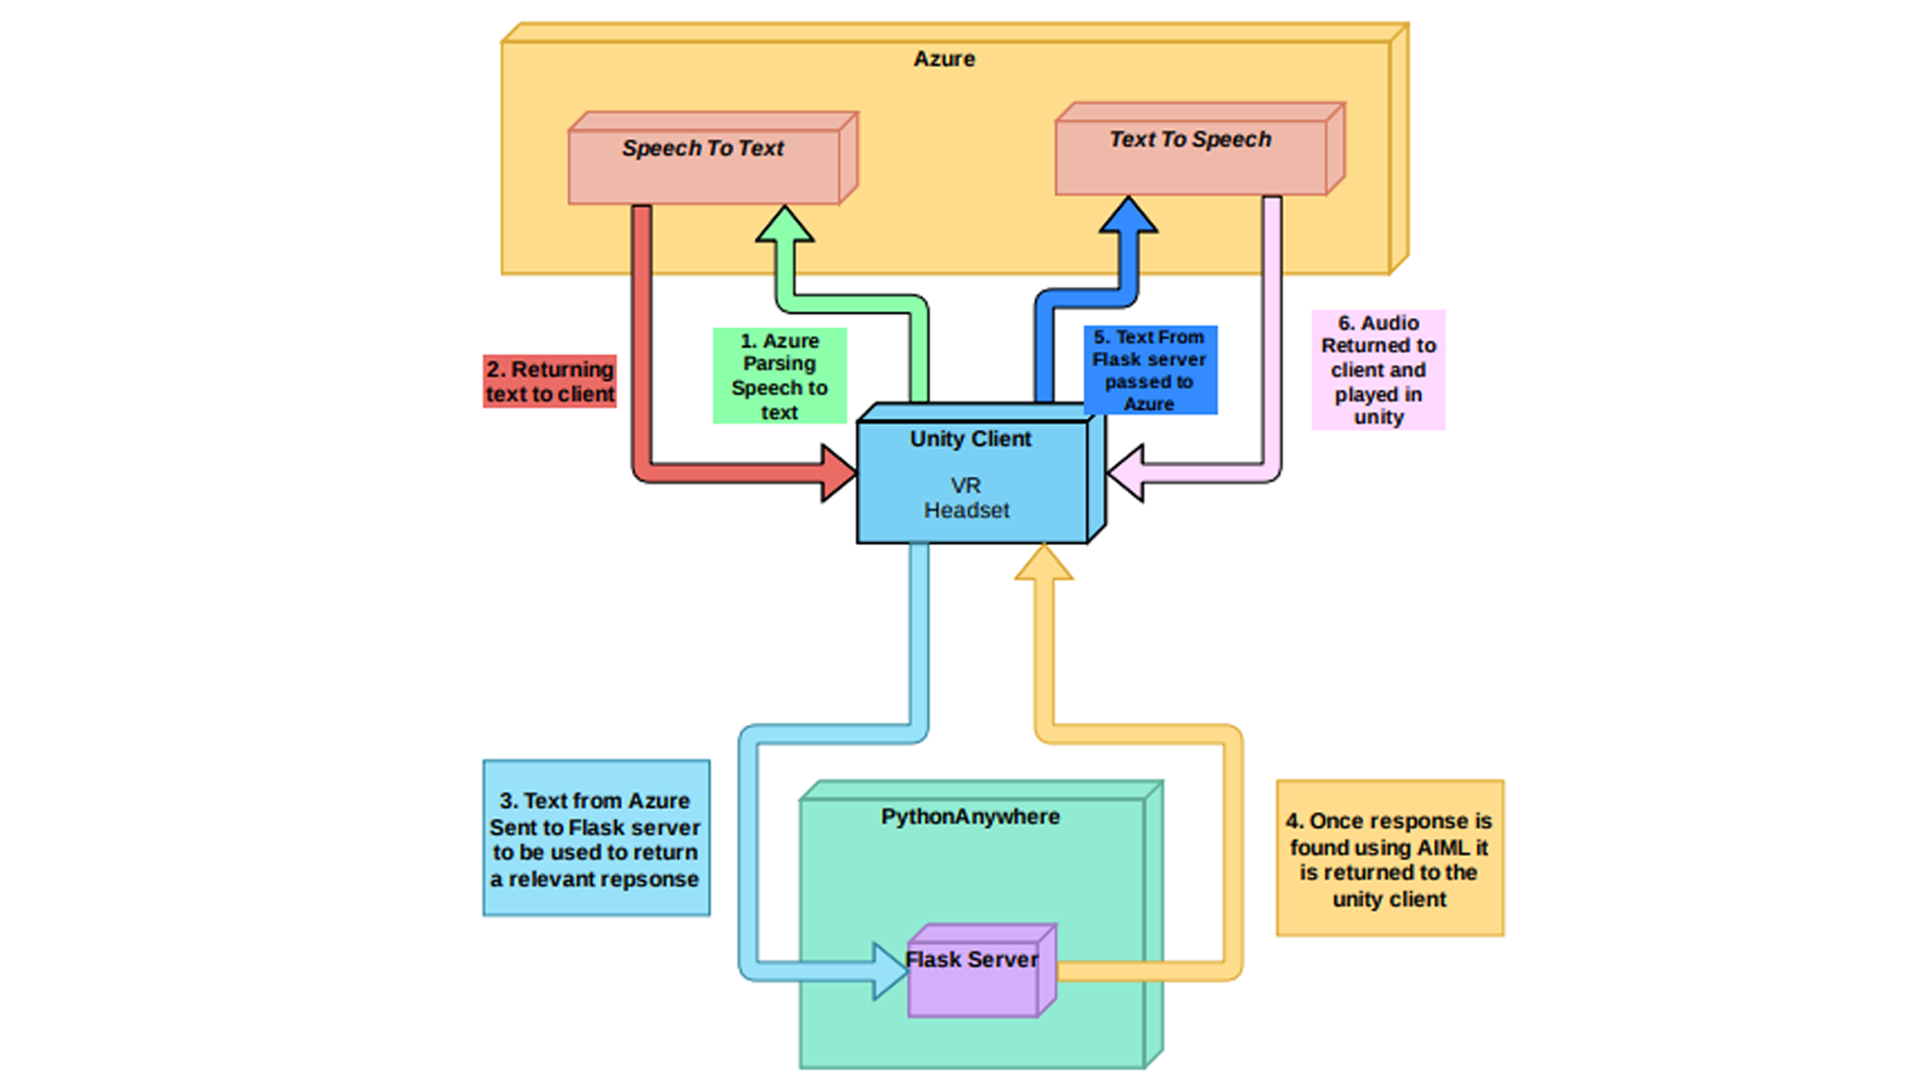
\includegraphics[width=1\textwidth]{Images/uml2.png}
\end{figure}

\section{Unity}
As seen in Figure~\ref{image:SystemArch} Unity is the central component in this application. It is the part that the user interacts with and the part where all the data flows in and out of. Having said that, in this section we will discuss the more graphical side of the implementation and how we did that.

\subsection{3D Models}
Generating realistic bots with realistic models was a problem that was easily solved with the aid of a website called "http://mixamo.com/". This website has an plethora of high quality 3d character models along with animations. Once the model was imported into Unity all that was left to do was give these bots a session ID,random voice, gender based on that voice and a random persona e.g Polite,neutral and rude. These personas would aid us later in deciding which AIML file to use server-side. As seen in Figure~\ref{fig:npcgen1} this is how we generate all these traits. The session ID is a random number between 1 and 10000. The persona is a integer between zero and three, each number meaning a different persona: 
\newline
\begin{table}[!ht]
    \centering
\begin{tabular}{ |p{3cm}|p{5cm}|  }
\hline
\multicolumn{2}{|c|}{NPC Personas} \\
\hline
Number & Persona \\
\hline
0 & Rude NPC \\
\hline
1 & Neutral NPC \\
\hline
2 & Polite NPC \\
\hline

\end{tabular}
    \caption{Personas}
    \label{tab:my_label}
\end{table}
\newline

Once these traits have been generated all that is left to be done is to generate them in the virtual 3D enviroment. The solution to this can be seen in Figure~\ref{fig:npcgen2}.
This snippet is also wrapped in a for loop to generate multiple random NPCs. There is an array of manually place GameObjects in the virtual world. These GameObjects act as spawning points for a single NPC. Based on the NPCs voice a Male or Female model is loaded then it is spawned in the position of one of the spawn points according to the index of the loop. After this process is complete we see NPCs standing in all the spawn points. This is how all the NPCs/Bots are spawned in the application.

\begin{figure}[htbp]
	\caption{Generate NPC Traits.}
	\label{fig:npcgen1}
	\begin{lstlisting}[language=python]
    public void SetSessionId()
    {
        sessionId = UnityEngine.Random.Range(1, 10000);
    }
    public void SetPersona()
    {
        persona = UnityEngine.Random.Range(0, 3);
    }
    public void SetVoice()
    {
        //0 = male 1= female
        int gender = UnityEngine.Random.Range(0, 2);
        Debug.Log("GENDER:" + gender);
        string[] voicesMale = {"en-US-GuyNeural", "en-IE-Sean"};
        string[] voicesFemale = { "en-US-JessaNeural", "de-DE-KatjaNeural" };
        if (gender == 0)
        {
            int rand = UnityEngine.Random.Range(0, voicesMale.Length);
            voiceName = voicesMale[rand];
        }
        else if(gender == 1)
        {
            int rand = UnityEngine.Random.Range(0, voicesFemale.Length);
            voiceName = voicesFemale[rand];
        }
    }
\end{lstlisting}

\caption{Generate NPCs In Virtual World.}
\label{fig:npcgen2}
\centering
\begin{lstlisting}[language=python]
    if (copy.GetComponent<NPC>().GetVoiceName() == "en-US-JessaNeural" || copy.GetComponent<NPC>().GetVoiceName() == "de-DE-KatjaNeural")
    {
        int rand = UnityEngine.Random.Range(0, 2);

        if(rand == 0)
        {
            copy = Instantiate(npc2, new Vector3(NPCSpawners[i].position.x, NPCSpawners[i].position.y, NPCSpawners[i].position.z), Quaternion.Euler(0, NPCSpawners[i].rotation.eulerAngles.y, 0));
            copy.GetComponent<NPC>().SetVoice(npcVoice);
            copy.transform.parent = container.transform;
        }else if(rand == 1)
        {
            copy = Instantiate(npc3, new Vector3(NPCSpawners[i].position.x, NPCSpawners[i].position.y, NPCSpawners[i].position.z), Quaternion.Euler(0, NPCSpawners[i].rotation.eulerAngles.y, 0));
            copy.GetComponent<NPC>().SetVoice(npcVoice);
            copy.transform.parent = container.transform;
        }
    }
    else
    {
        copy = Instantiate(npc1, new Vector3(NPCSpawners[i].position.x, NPCSpawners[i].position.y, NPCSpawners[i].position.z), Quaternion.Euler(0, NPCSpawners[i].rotation.eulerAngles.y, 0));
        copy.GetComponent<NPC>().SetVoice(npcVoice);
        copy.transform.parent = container.transform;
    }
\end{lstlisting}
\end{figure}

\subsection{Animation}


\section{HTTP}
\section{Oculus Quest}

\section{Azure}
\subsection{Azure Speech-to-Text}
\subsection{Azure Text-to-Speech}


\section{AIML}
% NEED THIS LATER
\begin{figure}[!h]
    \centering
    \begin{lstlisting}[language=PYTHON]
@app.route('/request', methods=['POST'])
def predictResponse():
    # Get json from request.
    sessionId = request.get_json()['sessionId']
    persona = request.get_json()['persona']
    userInput = request.get_json()['userInput']
    print(sessionId)
    print(persona)
    print(userInput)

    # Load specific aiml file depending on persona.
    kernel.respond("load aiml " + str(persona))

    print("DATA:")
    print(kernel.getPredicate("usersName", sessionId))

    # Predict reponse for specific session using user input.
    response = kernel.respond(userInput, sessionId)
    print(response)

    return response

\end{lstlisting}
    \caption{Caption}
    \label{fig:my_label}
\end{figure}


\section{Flask}

\section{PythonAnywhere}

\section{MongoDB}